\chapter[AR geometry and determinant relations]{Almost-split geometry, Hom control and determinant relations}
\label{arb:chapter}

The infinite locally gentle algebra and its completed order are the primary
objects in this chapter. Finite algebras enter through specified quotients or
special fibers, with their categories named. This distinction makes the pictures
more useful: a mesh is an exact sequence in an actual category, a tube is an
entire component, and a diagram of limiting words records additional objects
rather than suggesting an unproved equivalence.

We work over an algebraically closed field $k$ of characteristic zero unless
stated otherwise. Paths are written in travel order, so $ab$ traverses $a$ first.
We use right projectives $e_iA$ with this convention. Column representations may
instead be read over the opposite algebra; all displayed arrow-intertwining
identities use the usual column convention. This change of handedness does not
identify different categories or change any of the explicit Hom dimensions.

\section{What an AR picture specifies}
For an infinite polynomial dessin algebra $A=kQ/I$, write
$\operatorname{mod}_{\mathrm{fd}}A$ for finite-dimensional modules. Its arrow-adic
completion is $\Lambda=\varprojlim A/J^n$. A continuous finite-dimensional
$\Lambda$-module kills some $J^n$. A lattice over an order finite over
$R=k[[u]]$ is instead a finitely generated module free over $R$. A nonzero
lattice has infinite dimension over $k$ and is not a continuous finite-length
module. These distinctions persist even when the same quiver describes the
arrow actions.

The polynomial string classification has its own finiteness boundary.
For a finite quiver, finitely controlled modules are precisely finitely generated
modules: sum the finitely many finitely generated submodules containing their
vertex spaces. Pointwise artinian is likewise equivalent to artinian, by taking
a common stabilization index over the finitely many vertices. Thus
\cite[Theorems 1.2--1.4]{ARBCrawleyBoevey} genuinely applies to finitely generated
and artinian modules over our infinite polynomial string algebras, with its
specified strings, finite-dimensional bands and primitive injective bands.
It does not say that every module, or every infinite word, satisfies these
finiteness conditions.

A nonzero completed node lattice is outside both classes after restriction to
$A=k[x,y]/xy$. Indeed $A$ is finite over $k[u]$, $u=x+y$. If the lattice
were finitely generated over $A$, it would be finite torsion free over the PID
$k[u]$, hence finite free of positive rank. Multiplication by $1-u$ would then
have a nonzero cokernel. On a $k[[u]]$-lattice it is a unit, a contradiction.
The strictly decreasing chain $M\supset uM\supset u^2M\supset\cdots$ also
excludes artinianness. The lattice classification below is proved independently.

An almost-split sequence in an exact category is a nonsplit conflation
\[
 0\longrightarrow L\xrightarrow{i}E\xrightarrow{p}M\longrightarrow0
\]
whose first map factors every nonsection out of $L$ and whose second map factors
every nonretraction into $M$. Minimality removes redundant summands. The
Auslander--Reiten translate is $\tau M=L$. Irreducible maps give the arrows of
the AR quiver; projective vertices do not have nonsplit almost-split sequences
ending there. The mesh relation says that the two component composites, with
the appropriate signs, sum to zero. It is an identity between module maps.
It is not, without a further construction, a polynomial relation between
functions on a representation variety.

A quotient $A\twoheadrightarrow B$ gives a fully faithful exact inflation
$\operatorname{mod}B\to\operatorname{mod}A$. Its image is the full subcategory
annihilated by the kernel. That image need not be extension closed. Even when
it is closed under the relevant exact operations, an almost-split factorization
in the smaller category need not factor every map from the larger category.
Throughout, the word \emph{intrinsic} records this boundary.

\section{The corrected elliptic-theta face example}
\subsection{Permutations, genus and the actual algebra}
The six-dart data
\[
 \sigma=(1\,2\,3)(4\,5\,6),\qquad
 \alpha=(1\,4)(2\,5)(3\,6)
\]
are transitive and commute. With composition acting rightmost first,
\[
 \sigma\alpha=(1\,5\,3\,4\,2\,6),\qquad
 \phi=(\sigma\alpha)^{-1}=(1\,6\,2\,4\,3\,5).
\]
The uncontracted dessin has two black vertices, three white vertices, six edges
and one face. Thus $2-2g=2+3-6+1=0$, and $g=1$. After contracting the clean
white vertices the counts are two vertices, three edges and one face. A global
Belyi realization is $y^2=x^3-1$, $\beta=x^3$.

Its algebra has vertices $x_1,x_2,x_3$ and arrows
\[
 \begin{gathered}
 a_1:x_1\to x_2,\quad a_2:x_2\to x_3,\quad a_3:x_3\to x_1,\\
 b_3:x_1\to x_2,\quad b_1:x_2\to x_3,\quad b_2:x_3\to x_1.
\end{gathered}
\]
The forbidden travel pairs are
\[
 a_1b_1,\ b_1a_3,\ a_3b_3,\ b_3a_2,\ a_2b_2,\ b_2a_1.
\]
This is the same presentation as the corresponding right-to-left list after
reversing each product. For an explicit dart identification use
\[
 1\mapsto a_1,\quad2\mapsto a_3,\quad3\mapsto a_2,
 \quad4\mapsto b_3,\quad5\mapsto b_2,\quad6\mapsto b_1.
\]
Then the face is the forbidden indexing cycle
$a_1b_1a_3b_3a_2b_2$. It repeats vertices; it does not create six distinct
primitive idempotents. The algebra is infinite dimensional because its two
permitted three-cycles can be traversed indefinitely. Its completed order has
$R$-rank $18$.

\begin{proposition}[A face unfolds to a complex, not a six-vertex quotient]
\label{arb:unfold}
Put $B_6=k\widetilde A_5/J^2$, with the cyclic orientation. Every representation
of the theta algebra gives a $B_6$-representation by unfolding the face:
\[
 (V_1,V_2,V_3,V_1,V_2,V_3),\qquad
 (D_1,\ldots,D_6)=(a_1,b_1,a_3,b_3,a_2,b_2).
\]
The resulting functor is additive, exact and faithful, but is not full. There is
no unital surjection from this theta algebra to $B_6$.
\end{proposition}
\begin{proof}
Every consecutive product $D_{i+1}D_i$ is zero by the displayed relation list.
A theta morphism repeats its three vertex maps at the two corresponding face
positions, so it gives a complex morphism and is recovered from those repeated
maps. Kernels and cokernels are computed vertexwise, proving exactness and
faithfulness. On the vertex simple at $x_1$ its image is the sum of the two
$B_6$-simples at positions $1,4$. The original endomorphism space has dimension
one and the image endomorphism space dimension two. Thus fullness fails.

If a unital surjection to $B_6$ existed, compose it with
$B_6\twoheadrightarrow k^6$. Every theta arrow joins distinct idempotents.
Its image in this commutative algebra is therefore zero, since those two
idempotent images are orthogonal. The image is generated by the three vertex
idempotents and has dimension at most three, whereas a surjection to $k^6$
would have image dimension six. This is impossible.
\end{proof}

For a fixed theta dimension vector $(d_1,d_2,d_3)$, the arrays of six matrices
satisfying the equations are indeed the same affine variety as the circular
complex variety of dimensions $(d_1,d_2,d_3,d_1,d_2,d_3)$, after identifying the
repeated vector spaces and bases. The acting groups differ:
\[
 G_A=\prod_{i=1}^3\mathrm{GL}_{d_i},\qquad
 G_{B_6}=\prod_{i=1}^6\mathrm{GL}_{d_i},\qquad d_{i+3}=d_i.
\]
The first embeds diagonally in the second. Its orbits, Hom spaces and orbit
closures cannot be read by forgetting that diagonal restriction.
For example $a_1=1,b_3=\lambda$, all other arrows zero, gives pairwise
nonisomorphic theta representations when $\lambda\in k^\times$ varies.
Their unfolded complexes are all isomorphic: the two disjoint nonzero edge
maps may be rescaled independently by $G_{B_6}$.

\subsection{Correct rank strata and the incidence resolution}
The standalone circular-complex model remains valuable. Let $V_i=k^{d_i}$,
with indices modulo six, and set
\[
 \mathcal X(\mathbf d)=\{(D_i):D_i:V_i\to V_{i+1},\quad D_{i+1}D_i=0\}.
\]
A feasible rank vector satisfies
\[
 0\le r_i,\qquad r_{i-1}+r_i\le d_i.
\]
At each vertex choose a decomposition into the incoming image, a homology
space and an outgoing complement. Each outgoing complement maps isomorphically
onto the next incoming image. This proves that ranks classify orbits for the
\emph{six-factor} group. It also decomposes a complex into simple vertex modules
and length-two arrow modules. Thus $B_6$ is representation finite, with six
simples and six indecomposable length-two projectives; it is not the category
of the HLS diamond or of band tubes.

\begin{theorem}[Kernel incidence resolution]
\label{arb:incidence}
For a feasible $\mathbf r$, use subspaces of dimension $d_i-r_i$ and define
\[
 Z(\mathbf r)=\{(D,R):\dim R_i=d_i-r_i,\quad
       \operatorname{im}D_{i-1}\subset R_i\subset\ker D_i\}.
\]
This is smooth, and its projection is proper and birational onto the closure
of the rank-$\mathbf r$ stratum. The maximal feasible vectors, in componentwise
order, give the irreducible components of $\mathcal X(\mathbf d)$.
\end{theorem}
\begin{proof}
Over $\prod_i\mathbf{Gr}(d_i-r_i,V_i)$ the allowed maps are precisely
\[
 D_i\in\operatorname{Hom}(V_i/R_i,R_{i+1}).
\]
They form a vector bundle, so its total space is smooth and irreducible.
The incidence conditions are closed, and projection from the Grassmannian
product is proper. Its image is the locus of complexes with ranks at most
$\mathbf r$. To see surjectivity onto that locus, extend the incoming image to
a $(d_i-r_i)$-dimensional subspace inside the kernel; feasibility gives both
inequalities needed for that extension. Full ranks $r_i$ occur in the bundle,
since $r_i\le d_{i+1}-r_{i+1}$. On this open locus $R_i=\ker D_i$ is forced
and varies regularly, giving an inverse there. The image is consequently the
closure of this stratum. Every complex has a feasible rank vector and these
closures are ordered by componentwise rank, proving the last assertion.
\end{proof}
The index in $d_i-r_i$ matters. With all $d_i=1$ and the maximal vector
$(1,0,1,0,1,0)$, the alternative $d_i-r_{i-1}$ asks for a one-dimensional
$R_1$ inside the zero kernel of $D_1$. It has no fiber on the intended dense
stratum. This elementary counterexample rules out that incorrect resolution.
The theorem above describes the circular variety and its own group, not a
nonexistent quotient map of Proposition~\ref{arb:unfold}.

\section[Hom control and coverings]{Zwara's Hom control and covering Hom decompositions}
For finite-dimensional algebras $B,A$, an exact $k$-linear functor
$F:\operatorname{mod}B\to\operatorname{mod}A$ is \emph{Hom-controlled} in the
sense used by Zwara if there is a bilinear form
$\beta:K_0(B)\times K_0(B)\to\mathbb Z$ with
\begin{equation}\label{arb:homcontrol}
 \dim_k\operatorname{Hom}_A(FU,FV)-\dim_k\operatorname{Hom}_B(U,V)
       =\beta([U],[V])
\end{equation}
for all $U,V$. This is the explicit definition in
\cite[Section 6, p.71]{ARBRiedtmannZwara}, following \cite{ARBZwara}.
A fully faithful exact functor satisfies it with $\beta=0$, when these
finite-dimensional hypotheses apply. The definition does not consist of a
sum indexed by deck translates.

The face unfolding fails even this weaker numerical test on a finite
radical-square-zero quotient. Take dimension $(1,1,0)$, let $M_0$ have
$a_1=1,b_3=0$, and $M_1$ have $a_1=b_3=1$, all other maps zero. Their original
endomorphism dimensions are both one. After unfolding, $M_0$ has one edge
summand and two isolated simples, so its endomorphism dimension is three;
$M_1$ has two disjoint edge summands, so its endomorphism dimension is two.
The defects are two and one at the same $K_0$ class. No bilinear form in
\eqref{arb:homcontrol} can describe them.

Under suitable covering and support hypotheses a Galois push-down has the
separate identity
\[
 \operatorname{Hom}(F_\lambda M,F_\lambda N)
   \cong\bigoplus_{g\in G}\operatorname{Hom}(M,{}^gN).
\]
The support hypotheses ensure the asserted direct sum is the appropriate
space; an arbitrary infinite-support category may require other finiteness
conditions. Even when this formula holds, the nonidentity summands can depend
on the module structures rather than only on their $K_0$ classes.

\begin{proposition}[A finite covering counterexample]\label{arb:covercounter}
A Galois push-down need not be Hom-controlled in Zwara's sense, even for a
finite group and finite-dimensional algebras.
\end{proposition}
\begin{proof}
Let $B$ be the two-cycle $1\rightleftarrows2$ with all length-two paths zero,
and let $A=k[t]/t^2$. The deck involution exchanges vertices and arrows; the
quotient sends either arrow to $t$. Its push-down adds the vertex spaces.
Put $M=S_1\oplus S_2$ and $N=P_1$. Both have dimension vector $(1,1)$.
The first pushes to $k^2$ with $t=0$, the second to a single nilpotent Jordan
block of size two. Thus
\[
 \begin{array}{c|cc|c}
 &\dim\operatorname{End}_B&\dim\operatorname{End}_A(F(-))&\text{defect}\\\hline
 M&2&4&2\\N&1&2&1
 \end{array}
\]
while $[M]=[N]$ in $K_0(B)$. This contradicts any proposed bilinear defect.
The example satisfies the ordinary finite covering Hom decomposition; it is
the inference from that decomposition to \eqref{arb:homcontrol} which fails.
\end{proof}

The geometric conclusion must also be stated accurately. The module-scheme
result of \cite{ARBZwara} gives the specified smooth-then-immersion
factorization on connected components. The smoothness results for orbit
closures and rank schemes in \cite[Theorems 6.1--6.2]{ARBRiedtmannZwara} have
their own source, image and singularity-type hypotheses. They do not say that
every induced map into the entire module variety is smooth. For example the
quotient $k[t]/t^2\twoheadrightarrow k$ has fully faithful inflation, but the
point with $t=0$ is not a smooth immersion into the positive-dimensional
square-zero matrix variety in dimension two.

\section[Homogeneous tubes]{Homogeneous tubes in a polynomial dessin algebra}
Let $A=k[x,y]/xy$ be the actual polynomial interval dessin algebra. At the
smooth support $(x-\lambda,y)$, with $\lambda\ne0$, put
\[
 T_r=k[t]/t^r,\qquad x=\lambda+t,\quad y=0,\qquad r\ge1.
\]
All finite-dimensional modules at that support decompose into these modules.
This is the elementary divisor theorem for the nilpotent operator $t$.
Modules at different maximal supports have no nonzero maps between them.

\begin{proposition}[A full tube with explicit meshes]\label{arb:tube}
In $\operatorname{mod}_{\mathrm{fd}}A$ the $T_r$ form a homogeneous tube,
$\tau T_r=T_r$. With $T_0=0$ its sequences are
\[
 0\to T_r\xrightarrow{(\pi,t)}T_{r-1}\oplus T_{r+1}
      \xrightarrow{(t,-\pi)}T_r\to0.
\]
\end{proposition}
\begin{proof}
The two composites cancel. The first map is injective, including when $r=1$,
and the second is surjective; their dimensions then prove exactness.
A nonsurjective map into $T_r$ lands in $tT_r$ and factors through the first
summand of the right map. A surjective nonretraction from an indecomposable
$T_s$ has $s>r$ and factors through $T_{r+1}$. Decomposing a general source
proves right almost splitness; finite-dimensional duality proves the left
property. The sequence is nonsplit and its endpoints have local endomorphism
rings. Maps from other support blocks are zero, so this is an ambient
finite-dimensional-module assertion, not merely an intrinsic quotient claim.
\end{proof}

\begin{figure}[htbp]\centering
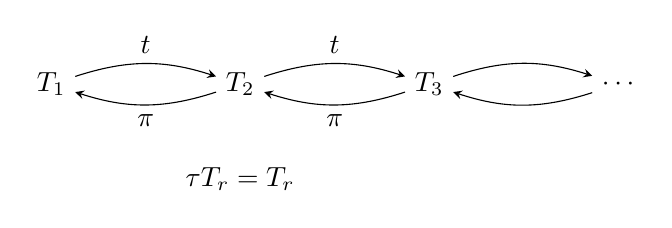
\begin{tikzpicture}[>=stealth,node distance=24mm]
\node (a) at (0,0) {$T_1$};\node (b) at (2.4,0) {$T_2$};
\node (c) at (4.8,0) {$T_3$};\node (d) at (7.2,0) {$\cdots$};
\draw[->,bend left=18] (a) to node[above] {$t$} (b);
\draw[->,bend left=18] (b) to node[below] {$\pi$} (a);
\draw[->,bend left=18] (b) to node[above] {$t$} (c);
\draw[->,bend left=18] (c) to node[below] {$\pi$} (b);
\draw[->,bend left=18] (c) to (d);\draw[->,bend left=18] (d) to (c);
\node at (2.4,-1.2) {$\tau T_r=T_r$};
\end{tikzpicture}
\caption{The entire rank-one tube, continued to every quasi-length. The
translation fixes quasi-length; the irreducible arrows change it.}
\end{figure}

The same construction is available on each branch of the polynomial theta
algebra at a nonzero central value. After inverting $u$, its algebra is the
product of two matrix algebras over $k[u,u^{-1}]$. Morita equivalence at a
fixed nonzero $\lambda$ gives one such tube on each branch, with dimension
vector $(r,r,r)$. Two arrows may be identities and the third $J_r(\lambda)$.
These are two \emph{families} indexed by $\lambda$, not two tubes in total.
They do not extend to continuous finite-dimensional completed-order modules:
there the central $u$ must be nilpotent.

There are also mixed inverse bands. Already $a_1b_3^{-1}$ is a primitive
cyclic string. More generally
\[
 (a_1a_2a_3)^j a_1b_3^{-1},\qquad j\ge0,
\]
has no forbidden subword in any power and is primitive because its cyclic
period contains exactly one inverse letter. Their different lengths give
infinitely many band classes. This disproves a classification by just the
two pure permitted triangles. Existence of these modules does not by itself
identify their entire ambient completed-order AR components.

At the singular central support, a pure-branch tube has only an intrinsic
meaning. The augmentation of the $y$-Jordan block $T_2^y$ onto $k$ cannot
factor through $T_2^x\to k$: any map $T_2^y\to T_2^x$ lands in
$\operatorname{ann}(x)=\operatorname{soc}(T_2^x)$, which that projection kills.
Thus even the first right almost-split factorization would fail in the larger
node finite-length category.

\section[Nodal lattice AR geometry]{The whole nodal lattice AR category and its stable triangles}
Let $\Lambda=k[[x,y]]/xy$, $u=x+y$, $X=(x)$ and $Y=(y)$. Normalize inside a
lattice's total quotient module using $B=k[[x]]\times k[[y]]$. If
$\overline M=BM$, the conductor gives
$u\overline M\subset M\subset\overline M$. The subspace
$M/u\overline M$ projects onto both branch residue spaces. Separate its pure
branch intersections and its common quotient; bases put it into pure lines
and diagonal pairs. Lifting those bases over the two DVRs gives
\begin{equation}\label{arb:nodeclassification}
 M\cong\Lambda^r\oplus X^a\oplus Y^b.
\end{equation}
This is a classification of the finite $R$-free lattice category. It is not a
claim that ordinary polynomial strings classify every completed lattice.

\begin{theorem}[The full nodal lattice meshes]\label{arb:nodear}
The two almost-split sequences in this category are
\[
 0\to Y\hookrightarrow\Lambda\xrightarrow{x}X\to0,
 \qquad0\to X\hookrightarrow\Lambda\xrightarrow{y}Y\to0.
\]
Its indecomposable lattice vertices are $\Lambda,X,Y$, with $\tau X=Y$, $\tau Y=X$.
\end{theorem}
\begin{proof}
The first kernel is $\operatorname{ann}x=Y$. It does not split: a map
$X\to\Lambda$ lands in $X$, and its composite with multiplication by $x$
is a nonunit of $\operatorname{End}X=k[[x]]$. Every map $\Lambda\to X$
factors through the displayed epimorphism, $\operatorname{Hom}(Y,X)=0$,
and each nonunit of $\operatorname{End}X$ is divisible by $x$, so factors
through $X\hookrightarrow\Lambda\to X$. Classification
\eqref{arb:nodeclassification} now proves right almost splitness for every
finite sum: a unit component from $X$ would already be a retraction.
For the left property, maps $Y\to X$ are zero, maps $Y\to\Lambda$
extend to multiplication on $\Lambda$, and each nonunit endomorphism of
$Y$ factors through $Y\hookrightarrow\Lambda\xrightarrow{y}Y$.
A unit component into a $Y$ summand would be a section. This proves the
factorization for every target in the classification. Endomorphisms of
$\Lambda$ fixing a structure map have constant term one, hence are units;
this proves minimality.
Interchange $x,y$ for the other sequence. There are no other nonprojective
indecomposables in this category.
\end{proof}

\begin{figure}[htbp]\centering
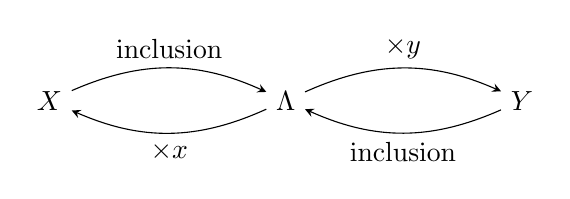
\begin{tikzpicture}[>=stealth]
\node (x) at (0,0) {$X$};\node (l) at (3,0) {$\Lambda$};
\node (y) at (6,0) {$Y$};
\draw[->,bend left=24] (x) to node[above] {inclusion} (l);
\draw[->,bend left=24] (l) to node[below] {$\times x$} (x);
\draw[->,bend left=24] (l) to node[above] {$\times y$} (y);
\draw[->,bend left=24] (y) to node[below] {inclusion} (l);
\end{tikzpicture}
\caption{The full lattice AR quiver. Its two opposite-branch mesh composites
are zero. The central vertex is projective.}
\end{figure}

Reduction by the regular parameter gives a genuine exact diagram:
\[
\begin{tikzcd}[column sep=large]
0\arrow[r]&Y\arrow[r,hook]\arrow[d,"u"]&\Lambda\arrow[r,"x"]\arrow[d,"u"]&X\arrow[r]\arrow[d,"u"]&0\\
0\arrow[r]&Y\arrow[r,hook]\arrow[d]&\Lambda\arrow[r,"x"]\arrow[d]&X\arrow[r]\arrow[d]&0\\
0\arrow[r]&k\arrow[r,"-\epsilon"]&k[\epsilon]/\epsilon^2\arrow[r]&k\arrow[r]&0 .
\end{tikzcd}
\]
All three terms are $R$-free, so the columns are exact and the free quotient
$X$ prevents a Tor term in the bottom row. With generators $y,x$ on the two
ends, $y=-\epsilon$ explains the sign. This diagram is stronger than a drawing
of four mesh diamonds with arbitrary rows and columns.

The lattice category is Frobenius. Alternating annihilator resolutions give
\[
 \operatorname{Ext}^1(X,\Lambda)=\operatorname{Ext}^1(Y,\Lambda)=0.
\]
The embeddings above give enough injectives, and $\Lambda$ gives enough
projectives. The projective-injectives are its finite free sums. Modulo them,
\[
 \underline{\operatorname{End}}(X)=
 \underline{\operatorname{End}}(Y)=k,\qquad
 \underline{\operatorname{Hom}}(X,Y)=
 \underline{\operatorname{Hom}}(Y,X)=0.
\]
For example maps through $\Lambda$ give precisely $xk[[x]]$ inside
$\operatorname{End}X=k[[x]]$. The two rows identify
$\Sigma X=Y$ and $\Sigma Y=X$. Hence its stable AR triangles are
\[
 Y\to0\to X\xrightarrow{\sim}\Sigma Y,
 \qquad X\to0\to Y\xrightarrow{\sim}\Sigma X.
\]
\begin{figure}[htbp]\centering
\begin{tikzpicture}[>=stealth]
\node (x) at (0,0) {$X$};\node (y) at (4,0) {$Y$};
\draw[->,dashed,bend left=25] (x) to node[above] {$\tau=\Sigma$} (y);
\draw[->,dashed,bend left=25] (y) to node[below] {$\tau=\Sigma$} (x);
\end{tikzpicture}
\caption{Stable node data: two isolated ordinary-quiver vertices. The dashed
arrows indicate translation and suspension, not irreducible morphisms.}
\end{figure}
The four ordinary arrows through $\Lambda$ disappear in the stable category.
A tube or a stable three-vertex grid would describe a different category.

\section[An HLS component in a dessin quotient]{A complete HLS component inside a genuine dessin quotient}
For $n\ge3$ take the infinite closed algebra with chain vertices $1,\ldots,n$,
endpoint loops $l,r$, opposite chain arrows $a_i,b_i$, and relations
\[
 l^2=r^2=a_ib_i=b_ia_i=0.
\]
Its single permitted cycle goes along the chain and back, with the endpoint
loops. It is an actual sphere dessin: the Chebyshev map
\[
 \beta_n(z)=\frac{1}{1-T_n(z)^2}
\]
has passport $(2n),(2^n),(2^{n-1},1,1)$; the dual contracted graph is a path.
Its completed order has rank $(2n)^2$. Kill one arrow at every chain edge,
retaining an orientation $\Omega$. The quotient is exactly $H_n(\Omega)$ of
\cite{ARBHLS}. A surviving path has length at most $n+1$, so the killed-arrow
ideal contains $J^{n+2}$. The polynomial algebra and its completion have the
same finite quotient. Denote its intrinsic module category by $\mathcal C_\Omega$.

For $H_3$ retain $1\xrightarrow a2\xrightarrow b3$. The following table fixes
all nine modules, not merely nine unlabelled points. A superscript $-$ denotes
a formal inverse, not an inverse in the algebra. Each word is read in travel
order; its basis consists of its successive visited positions.
\begin{center}\small
\begin{tabular}{c l c c}
\toprule Label&word&start&dimension vector\\\midrule
$A$&$l^-abrb^-a^-l^-$&1&$(4,2,2)$\\
$B$&$l^-ab$&1&$(2,1,1)$\\
$C$&$l^-abr^-$&1&$(2,1,2)$\\
$D$&$abrb^-a^-l^-$&1&$(3,2,2)$\\
$E$&$ab$&1&$(1,1,1)$\\
$F$&$abr^-$&1&$(1,1,2)$\\
$G$&$r^-b^-a^-labrb^-a^-l^-$&3&$(4,3,4)$\\
$H$&$r^-b^-a^-lab$&3&$(2,2,3)$\\
$I$&$r^-b^-a^-labr^-$&3&$(2,2,4)$\\\bottomrule
\end{tabular}
\end{center}
A direct letter sends the preceding position vector to the following one;
an inverse letter sends the following vector to the preceding one. These rules
satisfy $l^2=r^2=0$ and specify every arrow matrix.

\begin{figure}[htbp]\centering
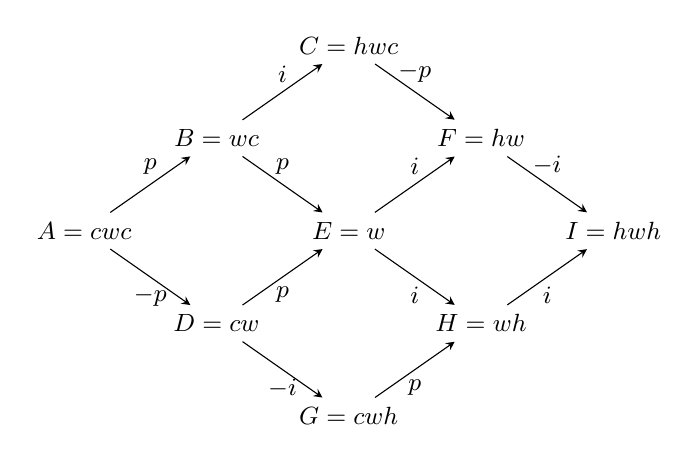
\begin{tikzpicture}[>=stealth,scale=.84, every node/.style={font=\small}]
\node (A) at (-4,0) {$A=cwc$};
\node (B) at (-2,1.4) {$B=wc$};\node (D) at (-2,-1.4) {$D=cw$};
\node (C) at (0,2.8) {$C=hwc$};\node (E) at (0,0) {$E=w$};
\node (G) at (0,-2.8) {$G=cwh$};
\node (F) at (2,1.4) {$F=hw$};\node (H) at (2,-1.4) {$H=wh$};
\node (I) at (4,0) {$I=hwh$};
\draw[->] (A)--node[above]{$p$}(B);\draw[->] (A)--node[below]{$-p$}(D);
\draw[->] (B)--node[above]{$i$}(C);\draw[->] (B)--node[above]{$p$}(E);
\draw[->] (D)--node[below]{$p$}(E);\draw[->] (D)--node[below]{$-i$}(G);
\draw[->] (C)--node[above]{$-p$}(F);\draw[->] (E)--node[above]{$i$}(F);
\draw[->] (E)--node[below]{$i$}(H);\draw[->] (G)--node[below]{$p$}(H);
\draw[->] (F)--node[above]{$-i$}(I);\draw[->] (H)--node[below]{$i$}(I);
\end{tikzpicture}
\caption{The actual signed HLS nine-object window, rotated to show four
meshes. Hook/cohook labels are operation labels from the source convention;
the preceding table fixes their travel words.}
\label{arb:diamond}
\end{figure}
The maps $p$ are projections and $i$ embeddings. In the rectangular version,
horizontal projections retain initial positions and horizontal embeddings
append the final $r^-$ position. Upper vertical projections delete the initial
$l^-$, and lower vertical embeddings prepend $r^-b^-a^-l$. The signs in
Figure~\ref{arb:diamond} give
\[
 \begin{gathered}
 0\to A\to B\oplus D\to E\to0,\qquad
 0\to B\to C\oplus E\to F\to0,\\
 0\to D\to E\oplus G\to H\to0,\qquad
 0\to E\to F\oplus H\to I\to0.
 \end{gathered}
\]
Their module intertwinings and exactness follow by these basis rules; for
example the two maps out of $A$ have joint kernel zero, the maps to $E$ are
onto, and the displayed dimension vectors give the kernel dimension at each
vertex. The almost-split property is the additional content of the source's
hook/cohook theorem, after identifying $w=ab$ as minimal of type $(2,2)$.

\subsection{Extending the window to the whole component}
Let $X_p$ mean $p$ left hooks when $p\ge0$ and $-p$ left cohooks when $p<0$;
let $Y_q$ mean $q$ right hooks when $q\ge0$ and $-q$ right cohooks when $q<0$.
These are operations on strings, not paths. Lemma 3.10 and the four-region
induction in \cite[Proposition 3.12]{ARBHLS} give every vertex of this component as
\[
 M(p,q)=M(X_p wY_q),\qquad (p,q)\in\mathbb Z^2.
\]
There are arrows increasing one coordinate at a time and
\[
 \tau M(p,q)=M(p-1,q-1).
\]
The meshes are
\[
 0\to M(p-1,q-1)\to M(p,q-1)\oplus M(p-1,q)\to M(p,q)\to0.
\]
The nine labels are $A=M(-1,-1),E=M(0,0),I=M(1,1)$ and the six intermediate
positions. This is the whole $\mathbb ZA_\infty^\infty$ component, continued in
all four directions. Its two outgoing axis rays are monomorphisms and its two
incoming axis corays epimorphisms. It is not an exact array of rows and columns.


\begin{figure}[htbp]\centering
\begin{tikzpicture}[>=stealth,x=2.7cm,y=1.35cm,every node/.style={font=\small}]
\foreach \p in {-1,0,1}{\foreach \q in {-1,0,1}{
 \node (m\p\q) at (\p,\q) {$M(\p,\q)$};}}
\foreach \q in {-1,0,1}{
 \draw[->] (m-1\q)--(m0\q);\draw[->] (m0\q)--(m1\q);
 \node at (-1.65,\q) {$\cdots$};\node at (1.65,\q) {$\cdots$};}
\foreach \p in {-1,0,1}{
 \draw[->] (m\p-1)--(m\p0);\draw[->] (m\p0)--(m\p1);
 \node at (\p,-1.65) {$\vdots$};\node at (\p,1.65) {$\vdots$};}
\draw[->,dashed] (m11) to[bend right=14] node[above,sloped] {$\tau$} (m00);
\end{tikzpicture}
\caption{The coordinate model of the entire HLS component: continue this
lattice for all $(p,q)\in\mathbb Z^2$. Ordinary arrows increase one coordinate;
translation decreases both. Only mesh diagonals give the exact sequences
above. The dashed arrow is translation, not an additional irreducible map.}
\end{figure}

The complete $H_n$ module AR inventory is also known
\cite[Theorem 3.14]{ARBHLS}: one component containing the projective and injective
modules; one exceptional tube of rank $n-1$; homogeneous band tubes; and the
components above indexed by minimal type $(2,2)$ strings. In $H_3$ the exceptional
tube has rank two. The source's Figures 3--4 show the projective-injective
component, not another view of this stable grid. None of these classifications
is silently asserted for every module of the completed infinite order.

\section[Derived AR triangles]{Derived AR triangles and an explicit infinite-pd endpoint}
A short exact sequence gives a triangle in a bounded derived category, but
almost splitness is tested against all objects there, including shifts.
For a finite-dimensional algebra an indecomposable endpoint admits a derived
AR triangle precisely when it is perfect; its translate is the derived
Nakayama functor followed by $[-1]$. In the finite-dimensional gentle setting,
\cite[Section 5.1]{ARBOPS} applies this criterion to finite homotopy strings and
bands, and describes the graded endpoint rotations. The finite-dimensional,
grading, boundary and local-system hypotheses remain part of that theorem.

For our $E=M(ab)$ the failure of perfectness can be seen directly. In the
travel/right convention the cover $P_1\to E$ has the eight-element basis
\[
 e_1,l,a,la,ab,lab,abr,labr,
\]
and retains $e_1,a,ab$. Its kernel is $lP_1\oplus abrP_3$.
Multiplication by $l:P_1\to P_1$ has kernel $lP_1$, since exactly the paths
already starting with $l$ are killed. The terminal simple repeats through
$r:P_3\to P_3$ in the same way. Thus its minimal projective resolution has
nonzero terms in arbitrarily high degrees. In particular the module AR sequence
ending in $E$ in Figure~\ref{arb:diamond} does not become an AR triangle ending
in $E$ in $D^b(\operatorname{mod}H_3)$.

By contrast, the smooth-support block of Proposition~\ref{arb:tube} is hereditary.
The operator $(x-\lambda)^r$ is a nonzerodivisor of the polynomial node algebra
and its cokernel is $T_r$, so it gives a length-one free resolution. The
indecomposables in that block's bounded derived category are $T_r[n]$; each
fixed shift has the same homogeneous tube and the AR triangles are induced
by its exact sequences. The nodal stable lattice triangles above give another
actual triangulated model. These two positive descriptions do not identify
all of $D^b$, $\operatorname{Perf}$ and the stable lattice category.

\section[Ringel's wind-wheel tile]{Ringel's wind-wheel tile: limits are part of the object}
Ringel's $\mathcal T(45)$ is the tile of the five-bar wind wheel specified in
\cite[Section 12.5, p.30]{ARBRingel}, drawn in Section 13.3, pp.38--40.
It is part of an AR \emph{quilt}, not just a finite-module mesh. Four finite-word
quarters surround a nonperiodic two-sided word. The diagonals consist of
one-sided limiting words; contracting ones use ordinary strings, expanding
ones need completion, and the central mixed word needs partial completion.
The five-tile example glues to a torus with five holes. Deleting the infinite-word
points recovers its finite string components. This is a category construction,
not an assertion that its quilt genus equals the genus of our original Belyi pair.

\begin{figure}[htbp]\centering
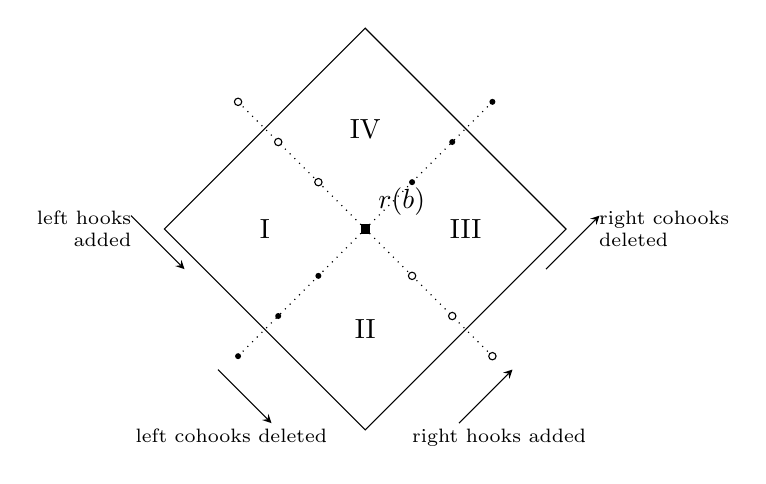
\begin{tikzpicture}[>=stealth,scale=.85]
\coordinate (n) at (0,3);\coordinate (e) at (3,0);
\coordinate (s) at (0,-3);\coordinate (w) at (-3,0);
\draw (n)--(e)--(s)--(w)--cycle;
\draw[dotted] (-1.9,1.9)--(1.9,-1.9);
\draw[dotted] (-1.9,-1.9)--(1.9,1.9);
\foreach \x in {.7,1.3,1.9}{
 \draw[fill=white] (-\x,\x) circle (.055);
 \draw[fill=white] (\x,-\x) circle (.055);
 \fill (-\x,-\x) circle (.045);\fill (\x,\x) circle (.045);}
\fill (-.07,-.07) rectangle (.07,.07);
\node[above right] at (.05,.05) {$r(b)$};
\node at (-1.5,0) {I};\node at (0,-1.5) {II};
\node at (1.5,0) {III};\node at (0,1.5) {IV};
\draw[->] (-3.5,.2)--(-2.7,-.6);
\node[align=right,left,font=\scriptsize] at (-3.35,0) {left hooks\\added};
\draw[->] (-2.2,-2.1)--(-1.4,-2.9);
\node[below,font=\scriptsize] at (-2,-2.85) {left cohooks deleted};
\draw[->] (1.4,-2.9)--(2.2,-2.1);
\node[below,font=\scriptsize] at (2,-2.85) {right hooks added};
\draw[->] (2.7,-.6)--(3.5,.2);
\node[right,align=left,font=\scriptsize] at (3.35,0) {right cohooks\\deleted};
\end{tikzpicture}
\caption{A scoped schematic of Ringel's tile, with the directions and limit
symbols of the primary picture: circles are contracting one-sided words,
bullets expanding ones, and the black square the two-sided limit. The border
and neighboring-tile identifications are additional data.}
\end{figure}

This picture is a finite-dimensional special-biserial wind-wheel category.
It is not already our completed node or the $H_n$ quotient. No map identifying
its algebra with a present dessin quotient has been supplied here. Such an
import would have to specify that map and the category in which almost-split
or pure-injective statements are retained. In particular deleting diagonals
from one tile leaves four quarters, not one HLS grid. Ringel also lists
indecomposable algebraically compact modules omitted from the quilt; it is not
itself a classification of all ordinary modules or all pure-injectives.

\section[Meshes and semi-invariants]{What meshes can and cannot say about semi-invariants}
\subsection{Presentation determinants and their exact scope}
Let $P_0=\bigoplus_i(e_iA)^{a_i}$, $P_1=\bigoplus_i(e_iA)^{b_i}$ and
$f:P_1\to P_0$. When the evaluated Hom map is square, chosen bases give
\[
 c_f(N)=\det\operatorname{Hom}_A(f,N),\qquad
 c_f(gN)=\prod_i\det(g_i)^{b_i-a_i}c_f(N).
\]
The action on coordinate functions has inverse weight. Put $M=\operatorname{coker}f$.
The kernel is $\operatorname{Hom}(M,N)$. If $f$ is the injective first map of a
short projective resolution, its cokernel after Hom
is $\operatorname{Ext}^1$ and higher Ext vanish. A general presentation keeps
its other cohomology. These distinctions are part of the semi-invariant
construction, not consequences of an AR drawing \cite{ARBSchofield}.

\begin{proposition}[A mesh whose determinant is a free generator]
\label{arb:freegenerator}
An actual dessin quotient has an almost-split mesh whose presentation
semi-invariant generates a polynomial algebra with no relation.
\end{proposition}
\begin{proof}
In the Chebyshev order above kill vertex3, both loops and the reverse arrow,
retaining only $a:1\to2$. This is the genuine continuous quotient
$B=k(1\to2)$. Its three indecomposables are $S_1,S_2$ and
$E=(k\xrightarrow1k)$, by rank decomposition of a linear map. Its sequence
\[
 0\to S_2\xrightarrow{i}E\xrightarrow{p}S_1\to0
\]
is almost split: a nonretraction to $S_1$ from these indecomposables factors
through $p$, and dually for $i$. At dimension $(1,1,0)$ the single arrow
coordinate $z$ transforms by $g_2/g_1$. The short projective resolution
$P_2\to P_1\to S_1$ gives the determinant $z$. Its semi-invariant algebra
is $k[z]$, with no algebraic relation among this one generator, although
$p i=0$ is a mesh relation.
\end{proof}
This quotient AR sequence is not ambient. A module supported at vertex1
with $l=J_2$ has a nonsplit epimorphism to $S_1$. Every map from it to $E$
has zero vertex1 component, because $E(a)=1$ while its own arrow $a$ is zero.
That epimorphism cannot factor through $E\to S_1$ in the larger category.

\begin{proposition}[The product theorem with its hypotheses]
Suppose $0\to M'\to M\to M''\to0$ is exact and $M',M''$ have resolutions
of length one by finite projectives. At a dimension vector where both end
presentation Hom matrices are individually square, compatible bases give
$c_M=c_{M'}c_{M''}$, up to the fixed basis sign.
\end{proposition}
\begin{proof}
Lift the projective cover of $M''$ through $M$. Its horseshoe kernel sits in
a split sequence of the two projective kernels, so the middle resolution
has differential $\left(\begin{smallmatrix}d'&\xi\\0&d''\end{smallmatrix}\right)$.
Applying contravariant Hom gives a triangular square matrix, with diagonal
the two prescribed Hom maps. Its determinant is their product.
\end{proof}
Total squareness alone does not give the two factors. In the $A_2$ mesh at
$(1,1)$, $S_1$ has balanced Euler value, but $P_1$ and $P_2$ do not. The
three individual Schofield factors are therefore not all defined there.
Nor is the infinite-pd $H_3$ object $E=ab$ eligible for the short-resolution
hypothesis just because it sits in a diamond.

\subsection{Relative nodal determinants really are multiplicative}
The lattice AR sequence of Theorem~\ref{arb:nodear} is split after forgetting
to $R$. It therefore has the canonical line comparison
\[
 \det_R\Lambda\cong\det_R Y\otimes_R\det_R X.
\]
For any compatible endomorphisms it gives
\begin{equation}\label{arb:nodedet}
 \det_R(1-TF_\Lambda)=\det_R(1-TF_Y)\det_R(1-TF_X).
\end{equation}
Indeed an $R$-splitting gives a triangular matrix. For every $\Lambda$-linear
endomorphism of $\Lambda$, multiplication by $f=a(u)+b(u)x$, the basis
$(y,1)$ makes that matrix and its two scalar actions explicit:
\[
 F_\Lambda=\begin{pmatrix}a&-b\\0&a+ub\end{pmatrix},
 \qquad F_Y=a,\quad F_X=a+ub.
\]
Both sides of \eqref{arb:nodedet} are $(1-Ta)(1-T(a+ub))$.
This is a determinant-functor statement after the specified passage to
$R$-perfect modules, not a nonexistent finite $\Lambda$-projective resolution
of $X,Y$. On applying $\operatorname{Hom}_\Lambda(-,Y)$ the map between
the first two $R$-lines is multiplication by $u$; its cokernel is
$\operatorname{Ext}^1(X,Y)=k$. Thus underived Hom is not exact on this AR row.

On the reduced continuous finite-length representation variety of the
one-vertex node, the ordinary semi-invariant ring is in fact just $k$.
Scalar matrices act trivially by conjugation, forcing a nonzero character
$\det^m$ to have $m=0$. The nilpotent filtration gives a one-parameter
conjugation degeneration to zero arrows, so all invariant regular functions
are constant. This coexists with the nontrivial lattice AR sequences and
the relative determinant identity; the target data differ.

\subsection{An inherited relation and a framed Pl\"ucker relation}
A genuine unframed relation is obtained by retaining both arrows
$a:1\to2$, $b:2\to1$ in a Chebyshev quotient and killing all other vertices
and arrows. At dimension $(1,1,0)$ its coordinate ring is
$k[a,b]/(ab)$. The two coordinates have opposite torus weights and are
semi-invariants. Their relation $ab=0$ comes from the inherited zero relation;
it was not deduced merely from a mesh picture.

For a richer example use the actual elliptic-square order. Its dessin has
$\sigma=(1\,2\,3\,4)$ and $\alpha=(1\,3)(2\,4)$; there is one face,
so $1+2-4+1=0$ gives genus one. The two quiver vertices are the two clean
edges. The four arrows form one permitted alternating four-cycle, with two
arrows in each direction; every mixed consecutive choice is forbidden. Put
$V_0=k^2,V_1=k^2$, set both reverse arrows to zero, and let the two forward
arrows have arbitrary matrices $X,Y$. These modules kill $J^2$ and therefore
extend continuously to the completed order. \emph{Frame the source} $V_0$:
the acting group in the next statement is only $\mathrm{GL}(V_1)$.
Write $Z=[x_1,x_2,y_1,y_2]$ and $p_{ij}=\det(z_i,z_j)$.

\begin{theorem}[A genuine framed generator relation]\label{arb:plucker}
All six $p_{ij}$ have target character $\det$, and their subalgebra is
\[
 k[p_{12},p_{13},p_{14},p_{23},p_{24},p_{34}]
 \big/(p_{12}p_{34}-p_{13}p_{24}+p_{14}p_{23}).
\]
The stated quadratic is the full ideal of relations of these six functions.
\end{theorem}
\begin{proof}
On the dense open $p_{12}\ne0$, express the other columns in the basis
$x_1,x_2$ and expand determinants. This gives the quadratic; polynomial
continuation proves it everywhere. Conversely any nonzero six-tuple
satisfying it is realized by four columns. After choosing a nonzero $p_{12}$
by permutation, one may take
\[
\begin{gathered}
 z_1=(1,0)^t,\qquad z_2=(0,p_{12})^t,\\
 z_3=(-p_{23}/p_{12},p_{13})^t,\quad
 z_4=(-p_{24}/p_{12},p_{14})^t.
\end{gathered}
\]
Their last minor has the required value by the equation. The zero tuple is
also realized. The quadratic is irreducible: its nondegenerate quadratic
form has rank six, whereas a product of linear forms has rank at most two.
Its ideal is prime, so this image description proves it is the kernel of
the polynomial map on coordinate rings.
\end{proof}
The exact diagram behind decomposability is
$0\to\ker Z\to k^4\xrightarrow Z k^2\to0$ on the rank-two locus. Its
exterior comparison relates complementary kernel minors. The relation extends
to the lower-rank boundary; the diagram is not an almost-split sequence.

The framing is indispensable. With $X=I$ and
$Y=\left(\begin{smallmatrix}0&0\\1&0\end{smallmatrix}\right)$,
$p_{13}=1$, but swapping the source basis makes it zero. Thus $p_{13}$ is
not a semi-invariant for the full original source-and-target group.
The coefficients of
\[
 \det(X+tY)=p_{12}+t(p_{14}-p_{23})+t^2p_{34}
\]
are full-group semi-invariants. The framed six-generator relation must not be
misidentified as their unframed presentation.

\section[Physical and arithmetic scope]{What this supplies to the physical and arithmetic program}
The chapter supplies exact categories, explicit maps, parameter spaces and
some genuine determinant identities. These can organize an effective model's
states and couplings, but $\tau$ is a categorical translation, not by itself
a unitary time evolution or a self-adjoint Hamiltonian. A physical realization
must supply its Hilbert space, domain, positive metric and dynamics independently.
Likewise an arbitrary tube parameter is not a prime norm or a Frobenius eigenvalue.

A valid route from a mesh to polynomial functions requires a universal
family, the correct group action, determinant-admissible complexes and
rank hypotheses. A route from those functions to an arithmetic $L$-function
additionally requires descent, local factors, conductor and archimedean data,
convergence or regularization, and a determinant-preserving positive comparison.
The relative nodal identity and framed Pl\"ucker model give usable intermediate
constructions. They do not discharge those arithmetic or analytic obligations,
and no full GRH conclusion is asserted.
